All considered metrics are defined with the help of terms from a so-called confusion matrix as shown in Figure~\ref{fig:2_basics/4_metrics/1_confusion_matrix}. The matrix emerges from the general scenario in which predictions are made for a set of objects that can be either true or false. A prediction is true if its statement is consistent with reality about the object, also called ground truth, and false if the prediction contradicts reality. An example scenario would be an image recognition that has to determine whether a photo shows a cat or not. Then, four mutually exclusive types of predictions can be distinguished:

\begin{itemize}
    \item \textbf{\emph{True positives}} (TP) are predictions stating that a condition holds true when this is indeed the case. In the image recognition example, this would correspond to the case where the model correctly classifies a cat image as a cat.

    \item \textbf{\emph{False positives}} (FP) are negative predictions about objects where the condition is actually true, e.g. declaring an animal as cat although it is not. This type of error is also referred to as a \emph{Type 1 error}.

    \item \textbf{\emph{False negatives}} (FN) are another kind of erroneous predictions, also referred to as \emph{Type 2 errors}. They represent the case that an element with a true condition was classified as false - was overlooked, so to speak. An example would be a cat image not recognized as a cat.

    \item \textbf{\emph{True negatives}} (TN) are similar to true positives in that they are correct predictions, as well. They consist of rejective predictions about objects where the condition does indeed not apply, for example by recognizing that there is no cat in a cat-less photo.
\end{itemize}

Although it is generally desirable to obtain as many correct predictions as possible, true positives and negates are often differently important and errors of type one and two differently severe. In medicine, for example, not recognizing a disease could be much worse than accidentally diagnosing a healthy person as ill. Conversely, not recognizing guilt in a lawsuit might be less serious than convicting someone who is innocent. In the context of knowledge graph completion under the open-world assumption, the focus lies on true positives since the KGC model cannot make any qualified statements about non-applying facts without negative samples in the graph. Omitting a fact from the prediction only means that the model has too little evidence for that fact, not that it can falsify it.

\begin{figure}[t]
    \centering
    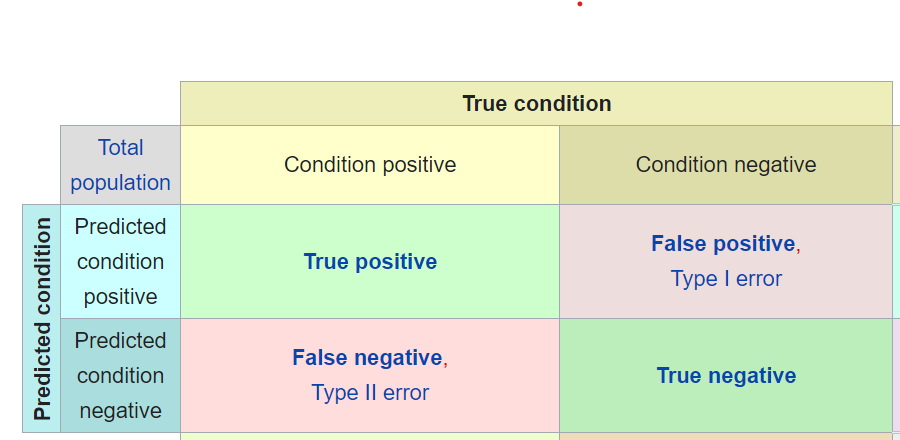
\includegraphics[width=\textwidth]{2_basics/4_metrics/1_confusion_matrix/matrix}
    \caption{Confusion Matrix}
    \label{fig:2_basics/4_metrics/1_confusion_matrix}
\end{figure}

"positive", "negative", "true", "false" predictions, "positive", "negative" elements

cat example
ir scenario
